
\section{Introduction}
\label{sec:org26ac92f}

Once underway, a wide variety of people will have in interest in tracking the progress of Rubin Observatory in making the Legacy Survey of Space and Time (LSST).
In some cases, the interest is general, focused primarily on understading whether is living up to expectations.
Many others will have more specific interests.
Scientists who will be using the data need both to understand what data is currently available, plan for what will be available in the future, and provide informed suggestions and feedback to the survey project. 
Members of the project itself will need to be able to identify problems and opportunities early, and adjust the survey's observing strategy accordingly.

Several Rubin Observatory planning documents recognize this need, and include related requirements:
\begin{itemize}
\item \href{https://ls.st/lse-29}{LSE-29}, the "LSST System Requirments Document," requires that the project "provide periodic status reports on the progress of the survey to allow both operations staff and the community to assess the survey progress" (LSR-REQ-0065), "create the necessary survey performance evaluation tools to predict the final results of the ten year survey based on the actual survey completed to date, assess the impacts of survey strategy changes resulting from changes in scientific priorities, and support the planning of the survey on a variety of time scales, from nightly through the entire 10 year duration" (LSR-REQ-0066), and "monitor the scientific and technical progress of the survey, communicate with the scientific user community and establish survey priorities, and adjust the survey design as needed to accomplish its goals given these priorities and achieved performance" (LSR-REQ-0070). Furthermore, LSE-29 describes the role of an Observing Scientist who will need tools for oversight of the data collection process, including intervention in the normally autonomous operations process (LSR-REQ-0071).
\item \href{https://ls.st/lse-30}{LSE-30}, the "Observatory Systems Specifications," repeats the requirement that the project "provide the tools and administrative processes necessary to monitor the progress of the ongoing survey, provide reports on the progress of the survey, respond to feedback from the science community, and evaluate the impact of changing science priorities over the 10 year survey lifetime" (OSS-REQ-0033), and create night summaries (OSS-REQ-131, OSS-REQ-0406), publish visits ahead of observing them (OSS-REQ-0378). In addition, LSE-30 has several other requirements for monitoring that are of interest for scheduling and progress purposes (OSS-REQ-0056, 0067, 0068, 0072, 0078, 0079, 0314).
\item the \href{https://docushare.lsst.org/docushare/dsweb/Get/Document-36797/Rubin\%20Observatory\%20Operations\%20Plan\%20April\%202020.pdf}{Rubin Observatory Operations Plan} of April, 2020 states that the System Performance department will "Ensure that the observing strategy being implemented by the scheduler software is on track to achieve its science requirements at the end of 10 years. Achieving this goal will involve simulating the remaining survey time; folding in an evolving understanding of the Observatory system and ascertaining whether a change to the Scheduling algorithm or configuration may be warranted. In addition to meeting basic survey requirements, it may be possible to maximize the breadth of science that can be done with LSST by making minor changes to the observing strategy. The (internal) Survey Evaluation Working Group will include representation from Observatory Operations and Data Production, and will evaluate quarterly the current and expected performance of the survey and scheduler (as analyzed by the Survey Scheduling Team) and make recommendations to the Director on any needed tactical changes to the survey cadence (e.g., due to impact of weather, telescope or data processing responses to the schedule, etc)."
\end{itemize}

Although they emphasize the need for progress monitoring for strategy optimization and describe some reports in which such information is to be reported, they do not specify the specific data, metrics, or plots to be used for such monitoring or included in these reports.
The specific set of diagnostics will evolve over the course of the survey, but three sources can guide the generation of an initial set:
\begin{itemize}
\item The formal requirments on the survey, for example as specified by LSE-29.
\item Metrics proposed by science collaborations for evaluation of survey strategy.
\item The experiences of precursor surveys such as the Sloan Digital Sky Survey (SDSS), Dark Energy Survey (DES) and the Zwicky Transient Facility (ZTF), in so far as there are relevant similarities between the surveys. Such experience can be useful both in what was these groups felt they did well, and what they wished they had done but did not.
\end{itemize}

Progress and strategy diagnostics (metrics, plots, and other figures) are usefully characterized by several features:
\begin{description}
\item[{Audience}] Different diagnostics and figures are useful to different audiences. Possible audiences include reviewers for and administrators of funding agencies, Rubin Observatory management, LSST science collaboration scientists, the Rubin Observatory Observatory Scientist, Observatory Support Scientists, Observing Specialists, Scheduler Scientists and Survey Software Engineers, astronomers working on other projects, other members of the astronomical community, and the general public.
\item[{Format}] The diagnostics may take any of serveral forms, including simple scalars, time series and other plots, maps, or other represntations of distributions.
\item[{Timing}] Diagnostics will need to be produced on range of timescale, ranging from hours to months. Some need to be produced shortly before or after each night of observing, or even periodically throughout the night. Others can be produced on a monthly schedule, or only in preparation for meetings and reviews.
\item[{Required data}] Data required to produce different diagnostics may originate in a variety of sources, including observatory telemetry, data products from Data Management, or sources outside the project (e.g. weather services).
\item[{Computing resources}] In some cases diagnostics can be produced with minimal calculation from available data sources. In other cases significant processing, up to and including suites of \texttt{opsim} simulations and corresponding calculation of metrics using \texttt{MAF}, will be required.
\end{description}

Each of these characteristics place requirements on the tools used to generate and provide access to the diagnostics.

\section{Metrics, plots, and other diagnostics}
\label{sec:orgd7ef0ca}
\subsection{Survey state descriptions}
\label{sec:orgba27bdd}
Figures and diagrams describing the current "state of the survey" will be of great interest to the community as a whole, and and providing an understanding of whether or not they correspond to the plan for the survey will be essential for explaining how well the survey is proceeding.
Examples of such diagrams will include:

\begin{description}
\item[{depth maps}] Maps of the survey showing the numbers of total visit, numbers of visits in each filter, and coadd limiting magnitude in each filter are likely to be the most prominant figures that show the current state of the survey. Current tools for evaluation of survey simulations produce examples of such plots, and \href{http://astro-lsst-01.astro.washington.edu:8081/allMetricResults?runId=392\#Basic\%20Maps}{results pages} show examples of such maps for the end of simulated surveys. Maps cut in an assortment of ways, for example including only visits with PSF widths narrower than some cutoff, may also be of interest. Figure \ref{fig:orga832664} shows an example of a depth map produced by MAF, for the end of a baseline survey.
\item[{depth/area plot}] A plot of the total area on the sky covered by the survey as a function of minimum depth will also be a useful representation of progress. Figure \ref{fig:orgf10554b} shows an example of such a plot produced by MAF, for the end of a baseline survey. When used to show survey progress, reference curves from a baseline simulation should be included as well.
\item[{filter use hourglass plots}] A single graphic that shows the distribution of filter use by time of night and year, and in relation to the moon, can indicate whether dark time is being used efficiently. The \href{http://astro-lsst-01.astro.washington.edu:8081/allMetricResults?runId=392\#Hourglass}{results pages} give examples of such plots for the ends of simulated surveys. Figure \ref{fig:orga357f6a} shows an example of such a plot produced by MAF, for the end of a baseline survey.
\item[{time use hourglass plots}] A single graphic that summarizes how time has been used by the survey so far will also be of wide interest. A plot will be a similar appearance to that of filter use hourglass plots, and like the plot will indicate time of year on one spatial axis and time of night on the other. Instead of indicating filter, however, this hourglass plot would indicate whether the pointing being observed corresponds to the FWD survey, a mini survey, or (if not science observing) what other activity was taking place. Likely categories to by symbolized by colors include: down time due to equipment failure, down time due to regular maintenance or engineering, down time due to weather, observing time without useful exposures (e.g. due to overcast skies), time spent on observations outside the WFD footprint (possible separated by mini-survey), time spent on DDFs, and other time in the WFD.
\item[{data quality hourglass plots}] A plot similar to the filter and time use hourglass plots, but uses the color coding to represent data quality (as measured by \(5\sigma\) limiting magnitude relative to nominal depth).
\item[{transient detection efficiency maps}] Maps of detection efficiency for different classes of variable objects (bright and faint near Earth objects (NEOs), TransNeptunian Objects (TNOs), Tidal Disruption Events (TDEs), fast microlensing events, type 1a supernovae, and others) over the footprint, for the entire survey so far and for the current season.\footnote{Gaps between seasons may be defined to be gaps between visits than include the date on which the sun has the same R.A. as the point on the sky.}
\item[{deep drilling field (DDF) cadence plots}] A set of plots (one for each DDF) showing the nights on which each DDF has been observed in the current season, and marking the time since it was last observed in each filter. Such plots may also encode the depth of exposures in each band on each night. Figure \ref{fig:org4c2c1e3} shows a sample cadence plot made using simulated data.
\item[{DDF transient efficienty plots}] The detection efficiency and actual numbers of detections for different classes of transients may be plotted as a function of date for each DDF. If these plots were combined with the DDF cadence plots, these plots may also guide an intuition for how gaps of different sizes affect the science for different classes of objects.
\end{description}

\begin{figure}[htbp]
\centering
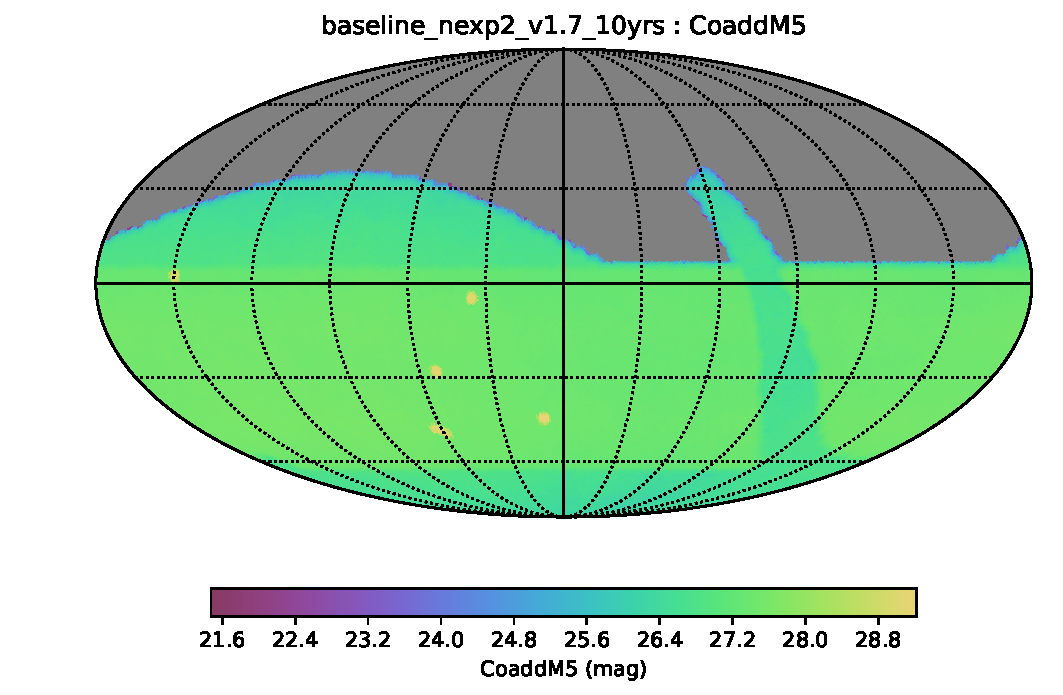
\includegraphics[width=.9\linewidth]{./figures/baseline_nexp2_v1_7_10yrs_CoaddM5_HEAL_SkyMap.pdf}
\caption{\label{fig:orga832664}Example depth map from MAF, for the state of the survey at the conclusion of the 10 year baseline simulation.}
\end{figure}

\begin{figure}[htbp]
\centering
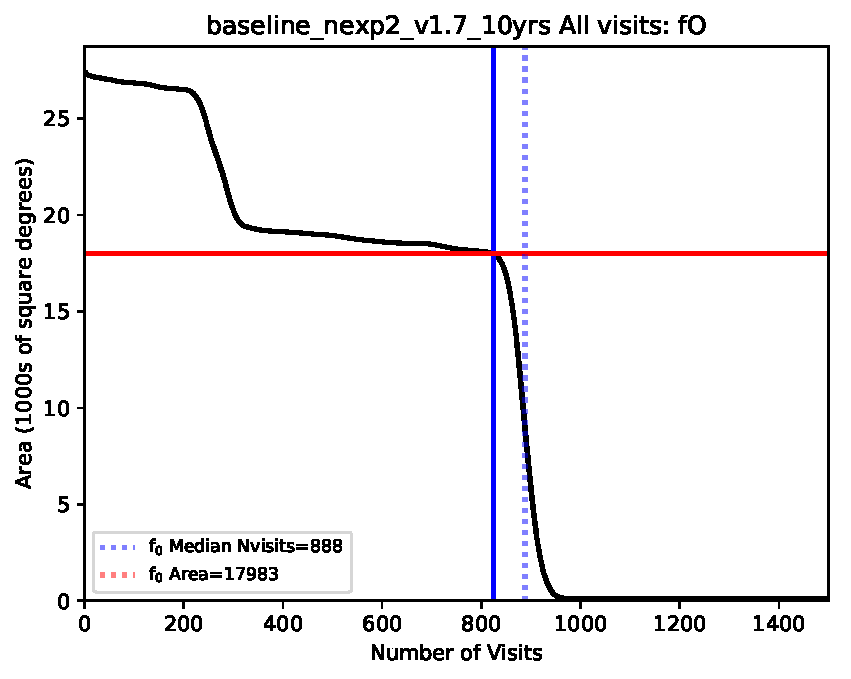
\includegraphics[height=0.4\textheight]{./figures/baseline_nexp2_v1_7_10yrs_fO_All_visits_HEAL_FO.pdf}
\caption{\label{fig:orgf10554b}Example depth-area plot from MAF, for the state of the survey at the conclusion of the 10 year baseline simulation.}
\end{figure}


\begin{figure}[htbp]
\centering
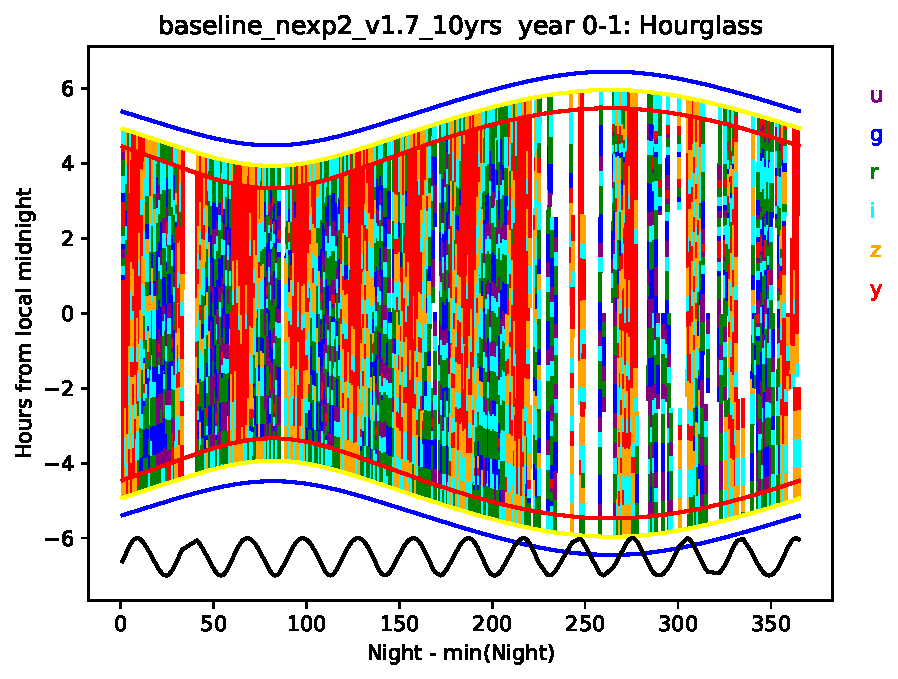
\includegraphics[height=0.4\textheight]{./figures/baseline_nexp2_v1_7_10yrs_Hourglass_year_0-1_HOUR_Hourglass.pdf}
\caption{\label{fig:orga357f6a}Example filter use hourglass plot from MAF, for the state of the survey at the conclusion of the 10 year baseline simulation. The black line along the bottom shows the lunar phase. The red and blue lines show nautical and civil twilight.}
\end{figure}

\begin{figure}[htbp]
\centering
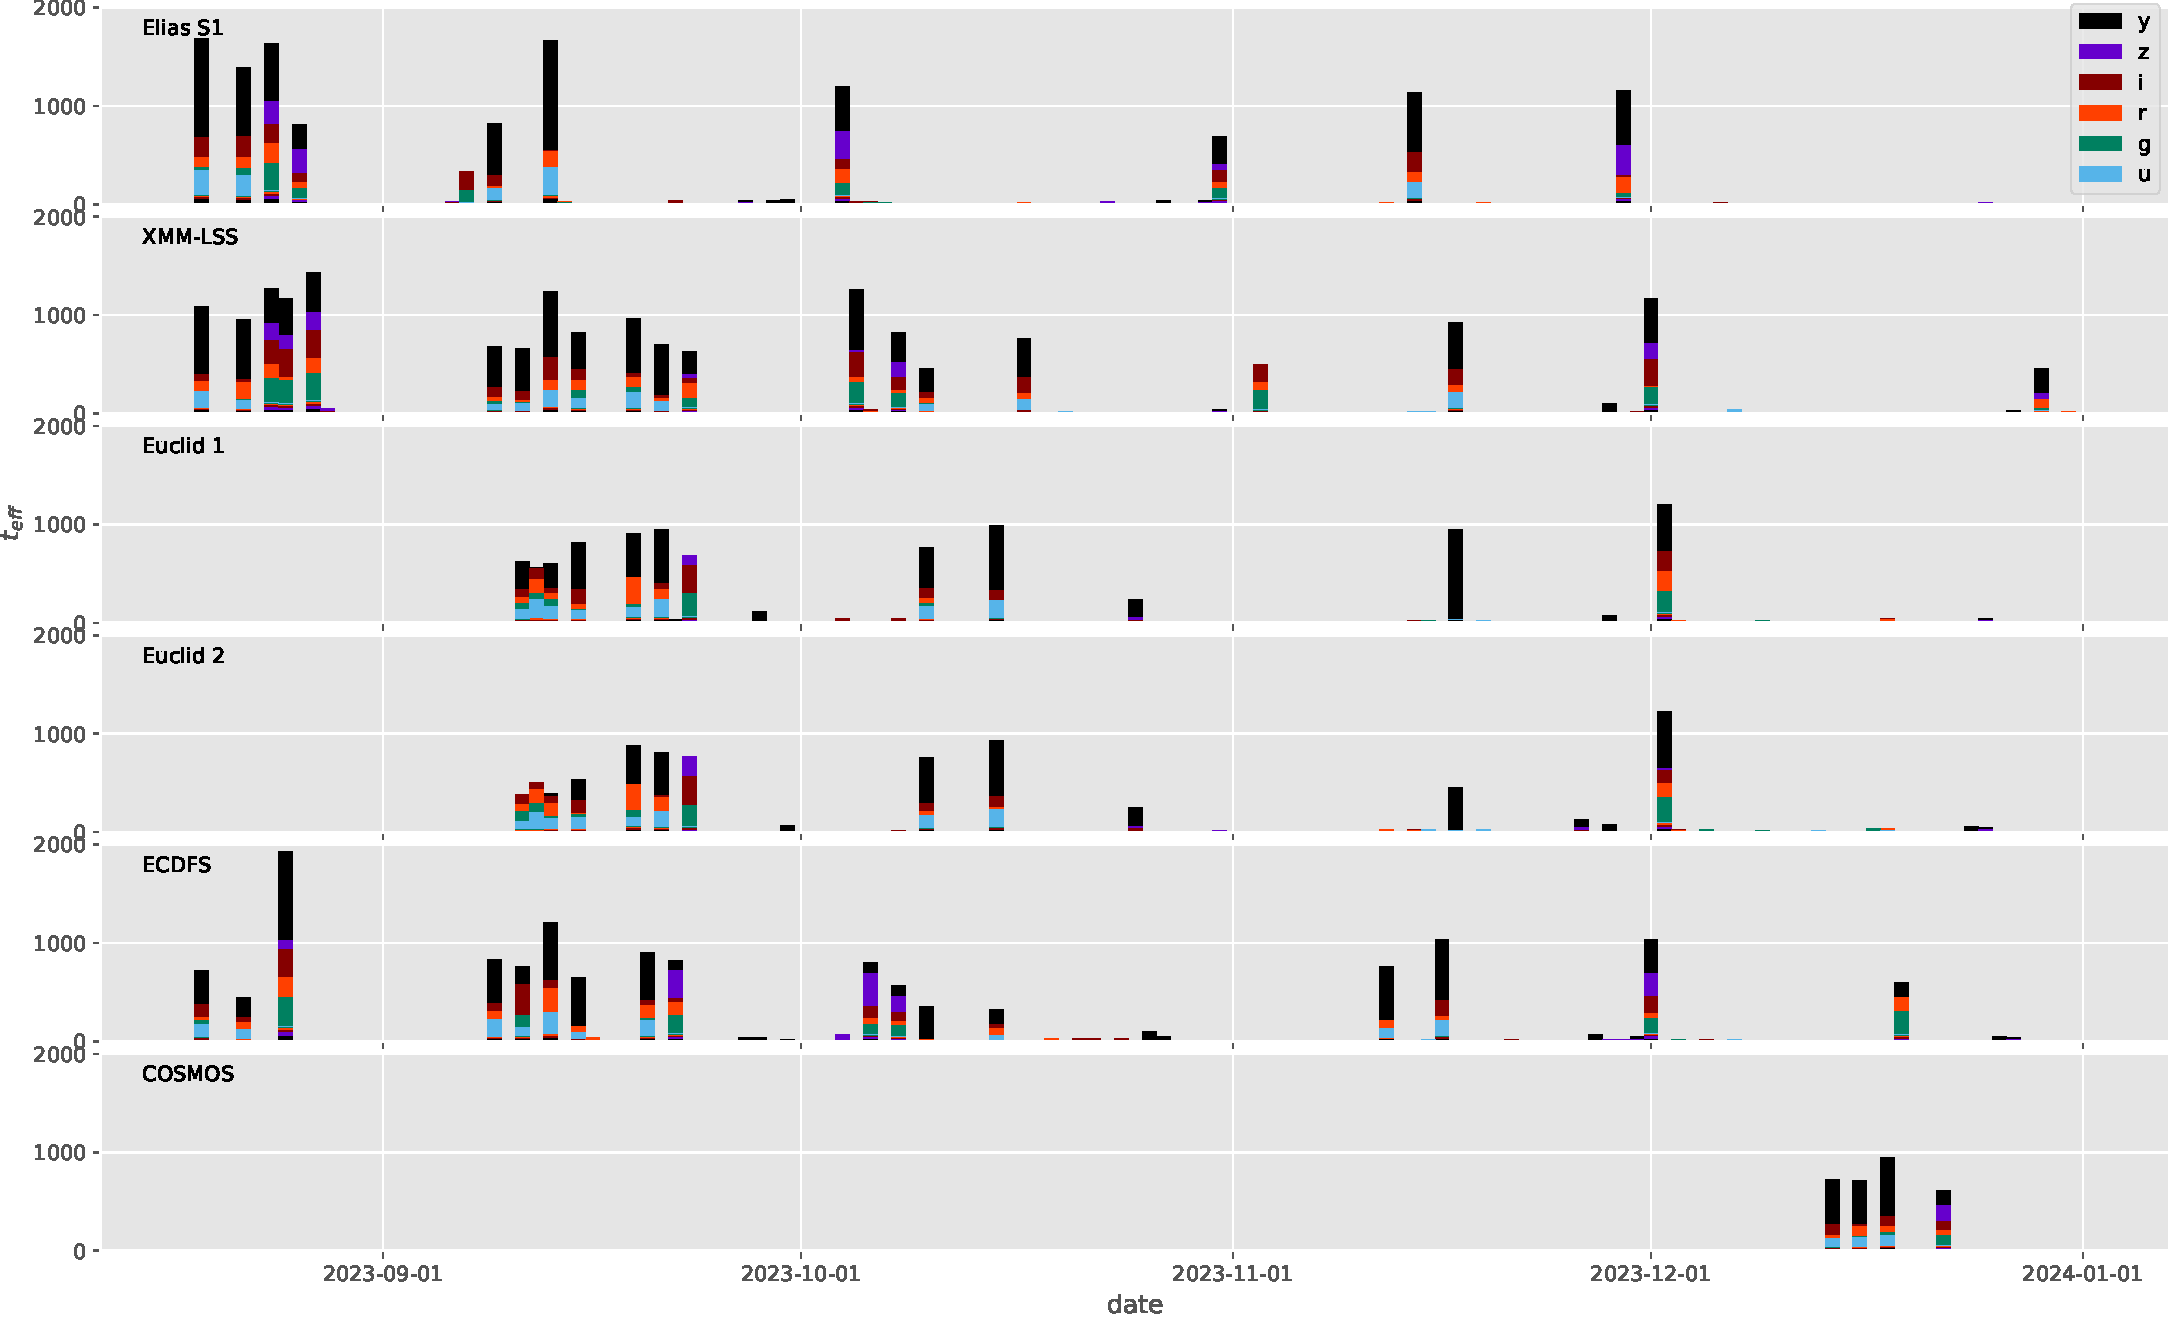
\includegraphics[height=0.4\textheight]{./figures/snhistory.pdf}
\caption{\label{fig:org4c2c1e3}A mock-up of an LSST DDF cadence plot, made using the version 1.7 baseline. Each subplot shows the cadence of a DDF field. The colors of the bars at each date represent different filters, and the heights of each color in each bar represents the combined effective exposure time, \(t_{eff} = 0.8 \times 10^{m5_{lim}-m_{0}}\), on that night in that filter, so that limiting magnitude of a coadded exposures from that night in that filter is \(m5_{lim} = m_{0} + \frac{5}{4} \log t_{eff}\).  In addition to the features shown in this mock-up, it would also be useful to show the nights of full moon, closest approach of the moon to each field, nights closed due to weather and other downtime, and time since the last set of visits deeper than some reference limiting magnitude.}
\end{figure}

\subsection{Time series progression of scalar survey metrics}
\label{sec:org63b5af6}
Many science metrics are expected to improve continuously over the course of the survey.
For each metric, there are two and perhaps three quantities that can be usefully compared:
\begin{description}
\item[{baseline}] the value of the metric for the given time, as measured from a reference simulation.
\item[{estimated}] the value of the metric for the given time, measured from the actually collected visits and visit parameters in the same way they were measured against the baseline simulation.
\item[{achieved}] the value of the metric as mearused from the final processed data products.
\end{description}

Estimated and achieved may differ in cases where the metric ultimately depends on the final catalogues of objects, which can only be estimated using the simple list of visits and data quality parameters produced by \texttt{opsim}.
One example of this would be the total number of stars and galaxies detected (PSTN-51 sections 3.3 and 3.6): errors and limited precision in the model for the distribution of stars and galaxies will result in a difference between the estimated and achieved values of the metric.

\begin{description}
\item[{Total, mean, median, min, max, and quantiles of numbers of visits}] Table 23 of \href{http://ls.st/lpm-17}{LPM-17}, "The LSST System Science Requirements Document," gives specifications for the "sum of the median number of visits in each band, Nv1, across the sky area". Additional statistics beyond the median are also indicative of the quality of the survey: highly skewed distributions, long tails to the distribution, or a significant difference between the mean and median could all indicate problems in scheduling. Good candidates for showing the time series of this distributions would be a time series boxplot or violin plot. See figure \ref{fig:org7ef55a6} for a sample created from the run 1.7 baseline simulation.
\item[{Numbers of science visits by band}] In addition to the sum across all bands, the distributions of visits in each band individually, and relative to each other, are also good indicators of whether the scheduler is behaving as expected. Time series plots of the visits split by band should rougly a constant proportionality on a timescale of months, but differences within each lunation, due to filters being swapped out and redder filters being preferentially chosen when the moon is very bright.
\item[{Numbers of science visits by R.A.}] Because the visibility of areas of the sky varies with the time of year, the distribution of visits across the sky is not expected to be uniform. Ideal visibility varies with R.A., so if the survey is ultimately to be uniform, the calendar observing dates elapsed and remaining need to corresponding rougly to the distribution of completed and needed visits for uniformity across the footprint. Plots of the number of visits in a set of R.A. bins as a function of date should show clear jumps at times when those R.A.'s correspond to local Sidereal times (LSTs) during the night in those times of year.
\item[{Numbers of science visits by program}] The fraction of time dedicatated to the Wide-Fast-Deep (WFD) survey and mini-surveys (including the Deep Drilling Fields (DDFs), Galactic Plane (GP), North Ecliptic Spur (NES), South Celestial Pole (SEP), and Target of Opportunity observations (ToOs)) will be specified as part the establishment of survey strategy, and whether the scheduler is adhering to these decisions should be monitored.
\item[{Science collaboration metrics}] \href{https://ls.st/pstn-051}{PSTN-51}, "Survey Strategy and Cadence Choices for the Vera C. Rubin Observatory Legacy Survey of Space and Time (LSST)," specifies a set of metrics contributed by the LSST science collaborations, including:
\begin{itemize}
\item detection completeness for different classes of transients and moving objects
\item numbers of stars and galaxies
\item the dark energy 3x2 Figure of Merit (FoM)
\end{itemize}
Supplements and refinements to these metrics are expected.
\end{description}

\begin{figure}[htbp]
\centering
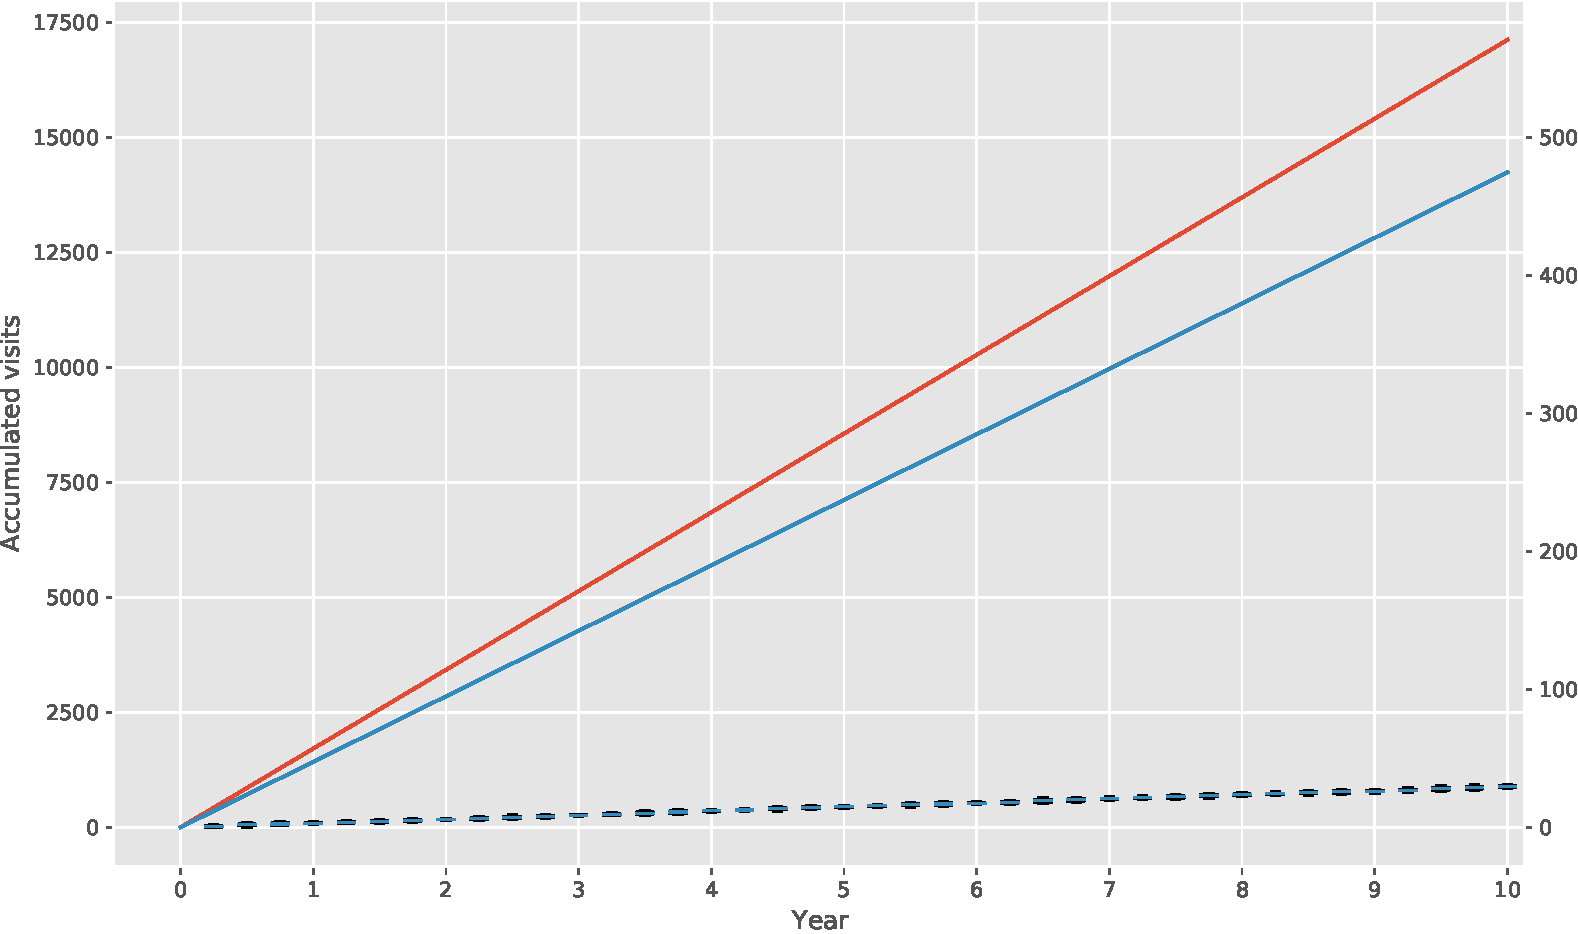
\includegraphics[width=.9\linewidth]{./figures/numvisits_boxplot.pdf}
\caption{\label{fig:org7ef55a6}Distributions of the number of visits in the best 18000 square degrees by year, for the the 1.7 2 visit baseline.}
\end{figure}

\subsection{Predicted scalar metrics for the final survey as a function of time}
\label{sec:orgf7b59ff}
Many survey metrics do not improve uniformly or even smoothly with time.
For example, the accumulated visits will be spread roughly uniformly over the survey footprint at any given time, so the area of sky observed to the nominal depth (specified in table 22 of \href{http://ls.st/lpm-17}{LPM-17}) will remain near zero for most of the survey, and then rise rapidly at the end: simply tracking the area covered to the nominal depth as a function of time does not provide a useful indication of progress being made toward achieving this metric.
Progress toward achieving this requirement can, however, be tracked using simulations: if the remainder of the survey is simulated after each night of observing and the final metrics measured using the final result, the time series can be plotted to indicate how much progress the survey is making in comparison with what is required.
A flat horizontal line will indicate a survey progressing exactly as expected based on simulations.
A rising line will indicate that the survey is making more progress than expected, while a falling one indicates that the survey is falling behind.

The final area is not the only metric for which these simulations are good tools for indicating progress; all of the scalar science metrics can be plotted in the same way. Plotting a selection of such metrics can show whether the current conditions or startegy are favoring some science goals over others in unexpected ways.
The list of metrics tracked this way should be the same as that in section \ref{sec:org63b5af6}.

\subsection{Nightly scheduler behaviour diagnostics}
\label{sec:org5918abd}
A number of plots and metrics will be needed to provide useful diagnostic information that can either help explain or predict the scheduler's behaviour, or identify potential problems in it.

These metrics can be usefully tracked at two times:
\begin{description}
\item[{start of night}] At least one \texttt{opsim} simulation should be run for the night before each night of observing. Nightly scheduler behaviour diagnostics should be calculated for these simulations, giving and indication of what is expected for the night, and providing advanced warning for any unexpected or anamolous behaviour. Nights of observing do not always proceed according to plan: slight differences in the start time or overhead between exposures may cause the predicted and actual schedule to diverge, and closures due to poor weather or equipment failure may create greater disruption. A handful of simulations with random offsets in start times and overheads between exposures can indicate the range of possibilities.\footnote{If the scheduler is modified to respond to observing conditions, then a handful of weather conditions will need to be simulated as well.}
\item[{end of night}] Nightly scheduler diagnostics should be calculated for each night shortly after the completion of observing. These diagnostics will alert the project to any scheduler problems or misbehaviour during the night, and help explain the scheduler's behaviour when it was not intuitive.
\end{description}

Examples of such diagnostics include:

\begin{description}
\item[{Feature maps}] Modern version of \texttt{opsim} select visits (or sets of visits grouped into "blobs") based on "features" that are functions of location on the sky: the slew time to reach the location on the sky, the expected depth of exposures to be taken there, and the progress made so far on that portion of the sky. A weighted mean of these features determines the selection of the next visit or set of visits. Examination of maps of these visits and the resultant final reward function is therefore fundamental to understanding the scheduler's behaviour. The presentation of the feature maps is complicated by the variablity with time and dependence on current pointing. Two candidate formats may be useful:
\begin{description}
\item[{animation}] a movie of the map over the night will provide the most detail, but can be difficult to navigate.
\item[{maximum feature values}] maps of the maximum value each point on the sky takes over the course of the night will be a useful indicator of how likely the scheduler is to schedule visits in these areas at some point in the night.
\end{description}
\item[{Full table of scheduled visits}] To support coordination between Rubin Observatory and other projects, \href{https://ls.st/lse-61}{LST-61}/DMS-REQ-0353 requires that "A service shall be provided to publish to the community the next visit location and the predicted visit schedule provided by the OCS. This service shall consist of both a web page for human inspection and a web API to allow automated tools to respond promptly." Such a table (in both forms) will be useful not only to external projects, but also to the observing scientists for understanding what to expect from the upcomming night, and for the Scheduling Scientists to catch potential issues with the scheduler.
\item[{Pointing movie}] A movie of the pointings of the telescope over the course of the night will be one of the fastest ways to convey an understanding of what the scheduler will do (before the night) or did (after it). Superposition of the pointings over the feature map.
\item[{Global observing efficiency}] The ratio of the total science exposure time to the available time (measured using morning and evening twilight as references) provides a good, gross indicator of whether the scheduler is scheduling visits efficiently (minimizing overhead time).
\item[{Gap distribution}] A histogram of the gaps in time between successive visits can indicate where inefficiencies in observing come from.
\item[{Table of long gaps}] Long gaps between exposures indicated either problems or inefficiencies. A short table of unusually long gaps between pairs of exposure with possible indicators of explanations (e.g. the slew angle between exposures, or whether there was a filter change) can call attention to this lost time for evaluation by a human.
\item[{H.A. distribution}] The distribution of hour angles for scheduled exposures indicates whether the scheduler is maximizing data quality.
\item[{DDF cadence plots}] The DDF cadence plots described in section \ref{sec:orgba27bdd} will also be important for understanding whether a DDF should be (or should have been) observed on a given night.
\item[{Fraction of time in blobs}] The "blob" scheduler is intended to be the workhorse scheduler for the WFD, and if an unexpectedly large number of exposures are being scheduled by the geedy scheduler, it may indicate a problem.
\end{description}

\subsection{Validation of the site and telescope model}
\label{sec:org4da74d3}
\texttt{opsim} simulations rely on several models for the characteristics of the site and the performance of the instrument.
Deviations from the models can have significant consequences for the accuracy of the simulations.
Comparisons between the modeled and achieved characteristics of the site and instrument will be important not only for understanding deviations between simulated and achieved performance, but also for improving simulations and making corresponding refinements to survey strategy.

For each modeled feature, there are at least two plots are of interest: one plots the measured values against the value calculated by the \texttt{opsim} model; and the other that tracks the distribution of residuals over time (for example a box or violin plot).
In some cases, additional plots may also be important.

Examples of modeled characteristics include:
\begin{description}
\item[{slew time}] In addition to simple compaing the modeled to achieved slew time, residuals between the two can be shown as a function of horizon coordinates and rotator angle.
\item[{filter change time}] Nominally 90 seconds plus up to 30 seconds to put the camera into the necessary position.
\item[{shutter time}] Nominally 1 second of overhead per visit.
\item[{readout time}] Nominally 2 seconds, in parallel with any slew time.
\item[{total overhead between successive exposures}] In principle the total overhead can be calculated by combining each source of overhead, but measurements of the total time from one exposure to the next (the start of of one visit to the start time of the next) will be an important diagnositic for discovering if the different values combine as expected, and if there are additional sources of overhead that have not been accounted for.
\item[{sky brightness}] The sky brightness as a function of airmass, sun and moon location and phase, filter, and other factors. Plots that show residuals with respect to horizon coordinates may also be useful for indicating limitations in the model due to light polution, which is not currently included in the model.
\item[{atmospheric seeing}] \texttt{opsim}'s simulation is based on achived data from the Gemini South DIMM. A comparison of the Gemini South and Rubin Observatory DIMM measurements will provide a diagnostic for resultanting limitations.
\item[{final delivered PSF width}] The final delivered PSF width is a function of the atmospheric seeing, filter, airmass, the turbulance outer scale, dome seeing, and other instrumental contributions. In some cases, the value used by the \texttt{opsim} model is highly uncertain (e.g. the turbulence outer scale). Other contributers (for example the effect of the strength and direction relative to the telescope pointing on the dome seeing) are not currently modeled at all.
\item[{extinction and lost time due to clouds}] The modules used for strategy simulation by \texttt{opsim} are based on historical cloud data recorded by humans at the nearby Cerro Tololo Inter-American Observatory. The correspondence between these estimates and actual time lost is highly uncertain.
\item[{time lost due to engineering activities and equipment failures}] 

\item[{achieved depth}] The expected \(5 \sigma\) limiting magnitude for point source detections in each visit is one of the basic "features" used by the scheduler, and is affected by a variety of factors. Comparisons between estimated and achieved depth are therefore of fundamental importance.
\end{description}

While some of these characteristics are functions of others, independent measurement of each will be important for verifying that the relations are those that are expected, and that there are no significant unaccounted for contributions.

In many cases, these characteristics will be tracked as part of telescope operations, independent of direct strategy considerations.
However, tracking and maintaining survey strategy requires presentation in a way that supports easy comparison to and updating of the \texttt{opsim} models.
Either the tracking and monitoring being done for other systems should include the necessary comparisons to the \texttt{opsim} models, or separate variations should be generated for the Scheduling Scientists and Survey Software Engineers.

\subsection{Disruption consequence analysis}
\label{sec:orgf8aac39}
The project will need to be able to quantify the consequences of departures from the final baseline strategy, both in advance and in retrospect. 
Possible causes of disruptions include "target of opportunity" observing and unexpected engineering downtime. 
It both cases, the consequences will not always be immediately obvious.
For example, a set of target of opportunity exposures will not necessarily result in complete loss of time for the WFD or other programs, because exposures scheduled for the ToO will often contribute to the FWD themselves. 
To quantify the effects of such disruptions, achieved metrics need to be compared to what they would have been without the disruptions.
This comparison requires additional simulations.
By comparing metrics derived from simulations in which the discruption never takes place with ones in which they did, both the immediate and long term effects of the disruption can be quantified.
The details of what simulations are needed for the comparison depend on whether the disruption being analyzed is one that has already occurred, or one which is under consideration or expected.
When evaluating possible future disruptions, the simulations for comparison are both simulations from the current time to the completion of the survey, differing only by whether or not the disruption occurs.
When evaluating the effects of a past disruption, the reference simulation (the one without the disruption) must begin in the past, before the disruption, and be run with the same environmental parameters (e.g. clouds and seeing) as actually achieved.
That way, the consequences of the disruption itself can be evaluated independentely of deviations between the simulated and actual survey.

In both cases, short and long term differences are of interest.
Two disruptions may have similar short-term effects on metrics, but some disruptions will be easier for the automatic scheduler to automatically recover from with future observations than others.
The time and degree to which it will be possible to recover from the disruption will sometimes be important information.

\section{Tools, reports, and their users}
\label{sec:orgf39aa30}
\subsection{Introduction}
\label{sec:org2d2a301}
The Rubin Observatory project and staff performing LSST will require survey progress and status diagnostics, including a variety of metrics and plots.
Some of these will be needed by the staff themselves, providing the data needed to prevent and diagnose problems, identify potential imporvements, and evaluate suggestions for changes.
In addition, such plots and metrics will also be needed for reports to the astronomical community and funding agencies, and even may be useful in engaging the general public.

The infrastructure suitable for producing such plots and metrics depend of several factors, including the audience expected to make use of them and the frequency with which they need to be produced.
Full automation of the production of plots and metrics will be most important when they need to be produced frequently, on a nightly or monthly basis.
When their audience includes non-experts, either full automation or simple production on demand will save effort.
Plots that are used primarily for debugging or exploration of specific issues may not require the same level of automation or simplicty of interface, but tools for reproduction of previous example of such diagnostics can be important for avoiding duplication of effort.

These plots and metrics can be produced and presented in any of several ways:

\begin{description}
\item[{Interactive tools}] When developing and debugging the software, hardware, and human procedures that produce the survey, experts working on the project require flexible tools to obtain and explore the relevant data. Planning and prediction of the consequences of events and choices will often benefit creation of simulations. Examples of such sets of tools (e.g. \texttt{opsim} and \texttt{MAF}) have been developed as part of project construction, and will continue to perform an important role in operations. General tools designed for monitoring other aspects of the survey (e.g. the health of the instrument or the status of data processing) will also have important roles to play.
\item[{Information dashboards}] Some plots and metrics will routine production and monitoring, often by those who are not expert users of the interactive tools like \texttt{MAF}. Even for those who do have the expertise, automation of the production of routine plots and metrics will save significant effort. Infrastructure that generates needed plots and metrics and presents them in a simple way (e.g. an automatically update web page, or small collection of web pages) will therefore be important. This infrastructure will require many of the same software components used by the interactive tools, plus some automation and presetation elements.
\item[{Reports}] The project will need to produce reports covering survey status and progress, whether in the form of documents and presentations. Many of the plots and metrics displayed in an information dashboard will be important elements in these reports.
\end{description}

The intended audience and the frequency of reporting are both important feature to consider in determining how any given metric or plot is to be generated.
Possible audiences include the funding agencies, Rubin Observatory management, LSST science collaboration scientists, the Observatory Science team (including the Observatory Scientist), the Observing Specialists, the Observatory Support Scientists, the Scheduler Scientists, Survey Software Engineers, astronomers working on other projects, other members of the astronomical community, and the general public. 
Plots and metrics may be generated on regular schedules (nightly, monthly, or quarterly), or as occasions demand.

The LSST system and data management requirements (\href{https://ls.st/lse-29}{LSE-29} and \href{https://ls.st/lse-61}{LSE-61}) and observatory systems specifications (\href{https://ls.st/lse-30}{LSE-30}) include requirements on several reports and reporting tools. The roles and activities in the \href{https://docushare.lsst.org/docushare/dsweb/Get/Document-36797/Rubin\%20Observatory\%20Operations\%20Plan\%20April\%202020.pdf}{Rubin Observatory Operations Plan} imply additional reports, and imply additional requirements on those already described.

\subsection{Night Plan}
\label{sec:org36f86b7}

Potential problems related to strategy or scheduling should be found and resolved before each night of observing, of possible, and the observing specialists on shift during the night need to be briefed and provided with a written plan describing any unusual activities or modes of operation, what they should expect of the scheduler, what behaviour they should consider anomalous, and how they should react to anomalous behaviour.
The \href{https://docushare.lsst.org/docushare/dsweb/Get/Document-36797/Rubin\%20Observatory\%20Operations\%20Plan\%20April\%202020.pdf}{Rubin Observatory Operations Plan} gives responsibility for reviewing and supervising scheduler behaviour to the Observatory Scientist and the Observatory Support Scientists, but specific procedures for this review and the briefing of the observing specialists are not yet developed.
Under any plan it would be worthwhile to automate the generation of the necessary scheduler simulations and diagnostics (listed in section \ref{sec:org5918abd}) for review and inclusion in briefing for the observing specialists and a plan for the night.

In operations rehearsals (summarized in \href{https://dmtn-119.lsst.io}{DMTN-119} and \href{https://dmtn-159.lsst.io/}{DMTN-159}), each night was planned in a daily meeting which included the current status and plans for the next night.
Among the "lessons learned" described in DMTN-119 was the need for a good note-taking during the daily meeting, with status report elements filled in prior to the meeting itself. 
The minutes of this meeting can then become a plan for the night.
Infrastructure to automate the creation of these report elements could either present them using a dashboard-like interface and be incorporated into the minutes, or create a template night plan directly, then supplemented during the meeting.\footnote{This process is similar to that used for observing for the Dark Energy Survey (DES).}

Automation in support of the night plan should include:
\begin{itemize}
\item Automatic creation of one or more scheduler simulations.\footnote{A side-effect of the creation of scheduler simulations completed in the afternoon is the creation of one or more candidate schedules. If these are produced in format that can be uploaded to the OCS, they can serve as a back-up to the scheduler in the unlikely event of a catastrophic failure of the scheduler during the night.}
\item Automatic creation of the diagnostics listed in section \ref{sec:org5918abd}, based on the simulations.
\item Presentation of the diagnostics a dashboard, automatically generated static report, or as part of a template observing plan for the night.
\end{itemize}

\subsection{Published upcomming schedule}
\label{sec:org91fab39}
To support coordination between LSST observing and that of other projects, including schedling of simultaneous or nearly simultaneous exposures the same areas of sky, the requirments specify that Rubin Observatory publish the observing schedule in advance.

One requirement that specifies the advanced schedule is \href{https://ls.st/lse-61}{LST-61}/DMS-REQ-0353, "Publishing predicted visit schedule":
\begin{quote}
Specification: A service shall be provided to publish to the community the next visit location and the predicted visit schedule provided by the OCS. This service shall consist of both a web page for human inspection and a web API to allow automated tools to respond promptly.

Discussion: The next visit and advanced schedule do not need to be published using the same service or protocol.
\end{quote}
another is \href{https://ls.st/lse-30}{LSE-30}/OSS-REQ-0378, "Advanced Publishing of Scheduler Sequence":
\begin{quote}
The scheduling of the observing sequence lasting at least \texttt{schedSeqDuration} shall be published in advance of each observing visit.
\end{quote}

These requirments imply the infrastructure necessary for:
\begin{itemize}
\item Automatic creation of scheduler simulations. The initial simulation for the night may be the same one as that described in section \ref{sec:org36f86b7}, but additional simulations throughout the night will also be required.
\item A service to publish the predicted schedule through a web API.
\item A service te publish the predicted schedule on a web page suitable for human inspection.
\end{itemize}

The overlap between these requiremnts and those for the creation of a night plan suggests that the same tool be used for both uses. 
Support for this use case imposes several additional requirements not present for the night plan:
\begin{itemize}
\item The published schedule and diagnostics must be available to the public, not just the project staff.
\item Update schedules need to be published as necessary though the night, not just at the start of the each night.
\item A web API suitable for support of automated tools must be supplied.
\end{itemize}

\subsection{Night reports}
\label{sec:orge04f42d}
Night reports (or nights summaries) are in important feature common to most astronomical facilities, and basic plots and metrics indicating survey progress are important elements for such reports in large surveys such as LSST.
Several Rubin Observatory requirements require specify different aspects of the content and creation of night reports, including LSE-30/OSS-REQ-0131, LSE-30/OSS-REQ-0406, LSE-61/DMS-REQ-0096, and LSE-61/DMS-REQ-0097. Section 1.4 of LST-490, the "Observatory Electronics Logging Working Group Report," acknowledges the need for infrastructure to support the creation of this report.
The specifications require that the report summarize "per system performance and behavior," but do not specify what is to be reported in great detail.
This report is a natural home for the nightly scheduler behaviour diagnostics (described in section \ref{sec:org5918abd}), when applied to actual (as opposed to simulated) scheduled nights.
Furthermore, some elements of the survey state description (section \ref{sec:orgba27bdd}) will be of broad enough interest that updates to them may be usefully included after each night.

In addition to the diagnostics directly related to scheduling, several of the data quality indicators that will be reported in the night report (following LSE-61/DMS-REQ-0097) to monitor the health of other subsystems are close to those needed for validation of the scheduler's site and telescope model (section \ref{sec:org4da74d3}). If these elements are produced with the needs of the scheduler scientists in mind, these same plots may fill both needs.

So, to support scheduler and survey progress monitoring, the night report should include:
\begin{itemize}
\item Comparisons of system characteristics (slew time, filter change time, depth, sky brightness, etc.) with models used by the scheduler simulator (some subset of the diagnostics listed in section \ref{sec:org4da74d3}).
\item Nightly scheduler behaviour diagnostics (most or all diagnostics listed in section \ref{sec:org5918abd}).
\item Updated diagnostics for the survey state (a selection of the diagnostics listed in section \ref{sec:orgba27bdd}).
\end{itemize}

\subsection{Tools for performance evaluation and analysis}
\label{sec:org34dba06}
The Observatory Scientist, Observatory Support Scientists, and the Survey Scheduling team will need to routinely monitor survey progress and assumptions at a more detailed level than supported by the night reports alone:
detailed monitoring will require all diagnostics listed in section \ref{sec:orgd7ef0ca}.
Furthermore, additional diagnostics will be required to debug specific problems, understand anomalies, and evaluate changing conditions or survey priorities.

In most cases, the different diagnostics will depend on a common set of data, including:
\begin{itemize}
\item observatory telemetry
\item one or more baseline survey simulations
\item the record of the visits completed up to and including the most recent night (including data quality information)
\item simulations of the future of the survey, starting with the next night of observing.
\item previously completed survey simulations, starting after each completed night of observing.
\end{itemize}

In some cases, analysis for scheduling and survey strategy may use tools developed for other purposes, such as maintenance of the instrument itself (as specified in \href{https://ls.st/lse-30}{LSE-30}/OSS-REQ-0067).
In other cases, analysis will require more flexible computation or access to data, including creation of custom scheduler simulations, access to archives of completed scheduler simulations, data management results, or even external data sources.
Once code for creation of a diagnostic is developed, the processes and tools used should support easy or automatic regeneration of the diagnostic.
When the creation is not computationally expensive, including it in a set of diagnostics to be automatically regenarated and posted nightly should be straightforward.
For computationally expensive diagnostics, inclusion in a set of diagnostics that can be repeated "on demand" should be similarly straightforward.

The set of tools available to the Survey Scientist, Survey Support Scientist, and the Survey Scheduling team should therefore include:
\begin{itemize}
\item APIs that provide access to observatory telemetry, archives of survey simulations, and DM output from within a common environment. These tools will therefore require access to either the summit Engineering and Facilities Database (EFD, \href{https://ls.st/sql-034}{SQR-034}) or the data management EFD (DM-EFD, \href{https://ls.st/sqr-029}{SQR-029}) for the telemetry data, and the DM butler for access to DM output. Access to an archive of past \texttt{opsim} simulations and the metrics calculated from them will also be required. That can be achieved by any of several means, including a simple filesystem.
\item A computational environment that includes the analysis and tools needed for computing diagnosits (e.g. jupyter notebooks with environments that include \texttt{opsim}, \texttt{MAF}, and stardard python scientific libraries)
\item Tools for automatic execution of lightweight code written to calculate diagnostics.
\item Tools for on-demand execution of computationally expensive diagnostic calculation.
\item A tool for collection and presentation of calculated diagnostics.
\end{itemize}

\subsection{Periodic progress reports and performance reviews}
\label{sec:orgdfa60c9}
The observatory staff and scheduling team will need to report progress and strategic concerns to management, funding agencies, and the community as a whole. Requirements for the existence of such reports are present in multiple plans and requirements documents. Some examples include \href{https://ls.st/lse-29}{LSE-29}/LSR-REQ-0065, "Survey performance reviews," which states:
\begin{quote}
The Observatory shall have the ability to provide periodic status reports on the progress of the survey to allow both operations staff and the community to assess the survey progress.
\end{quote}
and \href{https://ls.st/lse-30}{LSE-30}/OSS-REQ-0033, "Survey Planning and performance monitoring", calls out the need for reporting to the community at large:
\begin{quote}
The LSST shall provide the tools and administrative processes necessary to monitor the progress of the ongoing survey, provide reports on the progress of the survey, respond to feedback from the science community, and evaluate the impact of changing science priorities over the 10 year survey lifetime.

Discussion: It is expected that the performance of this task will require the use of detailed survey simulations in order to evaluate scheduling alternatives and optimize the future performance of the survey.
\end{quote}

The \href{https://docushare.lsst.org/docushare/dsweb/Get/Document-36797/Rubin\%20Observatory\%20Operations\%20Plan\%20April\%202020.pdf}{Rubin Observatory Operations Plan} gives responsibility for producing a quarterly report to the Observatory Support Scientist:
\begin{quote}
Responsible for producing a quarterly report on the scheduled/expected observations versus the performed observations. This analysis includes monitoring the assumptions used by the scheduler including slew times, shutter open/close times, readout times etc. 
\end{quote}

Multiple such reports will be made on different schedules, customized for different audiences.
All of these reports may draw from any of the report elements descibed in section \ref{sec:orgd7ef0ca}, but it is unlikely that any single report will require every element.
While the generation of individual elements will benefit from automation, the compilation and construction of such reports will require human attention and customization to each audience.

\subsection{Interfaces for education and public outreach}
\label{sec:orgc7b8c45}
While many survey progress metrics and visualizations are only likely to be of interest to experts, several will be intuitive, and may be good candidates for engaging the general public, as per \href{https://ls.st/lse-29}{LSE-29}/LSR-REQ-0113, "EPO Products, Tools, and Interfaces"
\begin{quote}
LSST EPO shall provide access to LSST data through tools, interfaces,
and learning experiences that are designedto engage communities with
different levels of knowledge, experience and skills.
\end{quote}
Good candidates for presentation to the public are movies of numbers of exposures generated, and plots numbers of galaxies (or other objects) detected as a function of time.
\section{Infrastructure needs}
\label{sec:org3f720f6}
\begin{description}
\item[{Data collection, storage, retrieval, and distribution}] Calculation of metrics and other diagnostics require a variety of data, including:
\begin{description}
\item[{summit telemetry data}] Telemetry data will be stored in the summit EFD and also a DM-EFD. Access to either of these through an API should be sufficient for strategy, scheduler, and progress monitoring needs.
\item[{data management results}] Some metrics such as total counts of stars and galaxies will require access to the results of data management. The DM butler is one option for such access.
\item[{simulation results}] The progress monitoring infrastructure will need an archive of \texttt{opsim} simulations, to which new simulations may be stored and from which old ones may be retrieved. Such results could potentially be stored a combination of the DM butler, but mechanisms such as a simple filesystem are likely to be adequate.
\item[{diagnostic results}] Metrics, plots, and other diagnostics will also need to be archived. These results could potentially be stored and and retrieved from the butler, and some of them may be suitable for a time series database such as that used by the EFDs, but such solutions may also be unnecessarily complex: a simple filesystem and small relational database are likely to be adequate for this task.
\end{description}
\item[{Data processing}] A handful of \texttt{opsim} simulations will need to be run after each night of observing, and a standard set of metrics calculated for them. Such simulations take a 6 to 8 hours to complete on 2020 hardware, so cannot be performed on demand. However, a simple single node with a cron job could adequately perform the task.
\item[{Dashboards and report generation}] Mechanisms for preseting the generated diagnostics and metrics will be required. For sets that should be reviewed daily, diagnostics  should be presented in pre-made sets according to their usage, without a need for the user to select or customize plots each time. For example, plots needed for the night plan and night report should be presented web pages or report templates without the need for human interaction or customization.
\end{description}

\section{Available infrastructure}
\label{sec:org0463fc9}
\begin{description}
\item[{opsim}] The existing scheduler software product already supports creation of simulations, and such capabilities will be maintained thoughout the life of the survey.
\item[{The Metrics Analysis Framework (MAF)}] MAF provides a collection of tools in python for the analysis of scheduler simulation results, and the science collaborations have developed (and are continuing to develop) metric calculation tools within this framework.
\item[{Engineering and Facilities Database (EFD)}] Observatory telemetry will be stored in EFDs. There are two EFDs under development: the summit EFD (\href{https://ls.st/LTS-210}{LTS-210}) and the Data Management (DM) EFD (\href{https://sqr-029.lsst.io/}{SQR-029}).  Data associated with validation of the site and telescope model used by the scheduler (section \ref{sec:org4da74d3}) will require access to one of these databases.
\item[{Data Management Butler}] The butler is the archiving and access tool that will be used by Data Management to store the results of processing. Calculation of several scheduler diagnostics will require access to this data. Examples include limiting magnitudes and other data quality measures and numbers of different types of objects detected (e.g. stars, galaxies). The butler appears to be flexibile enough to support storage of scheduler-related data sets, including the results of simulations themselves, but it is unclear that there are any advantages of storing such data in the butler rather than a simple file system.
\item[{Science Quality Analysis Harness (SQuaSH)}] SQuaSH (\href{https://sqr-009.lsst.io/}{SQR-009}) provides infrastructure for monitoring data management pipeline tasks. This infrastructure has many features in common with what is required for scheduling and survey progress related tasks. Elements of the SQuaSH infrastructure include (shown in the architecture diagram in SQR-009):
\begin{description}
\item[{execution environment}] SQuaSH includes a verification job execution environment.
\item[{time series database}] SQuaSH seems to be built around the assumption that each metric is best examined as a time series of scalar values. This is true for many progress and scheduling related metrics, but there are important exceptions, such as depth maps or distributions.
\item[{metric visualization}] SQuaSH includes an instance of \href{https://docs.influxdata.com/chronograf/v1.8/}{chronograph}, a timeseries visualization tool designed to work with the selected implementation of the time series database, \href{https://www.influxdata.com/products/influxdb/}{InfluxDB}. It seems likely that this tool would be useful for visualization of many of our time series metrics, but may lack the specialized visualizations present in existing tools like MAF, such as hourglass plots.
\item[{external dashboards}] 

\item[{Nublado}] 

\item[{nbreport}] SQuaRE includes infrastructure for running jupyter notebooks as templates for periodic reports, and uses the night report as a reference example (\href{https://sqr-026.lsst.io/}{SQR-026}). This system might be suitable for generation of the night plan, and as reports that can serve as first drafts for longer, less frequent reports.
\item[{S3 datastore}] 
\end{description}
\item[{faro}] 

\item[{LOVE}] 

\item[{Observatory Logging Ecosystem}] 
\end{description}
